% v2020-09-21

\documentclass[11pt,a4paper]{article} %coverpage uses 12pt
\usepackage[utf8]{inputenc}

\usepackage{fancyhdr} % Fancy headings
\usepackage{amsmath} % mathematical features 
\usepackage{multirow}
\usepackage{xspace}
\usepackage{longtable}
\usepackage{rotating}
\usepackage{listings} % source code printing
\usepackage{hyperref} % links in pdf
\usepackage{booktabs,colortbl} % more commands for tables and coloring
\usepackage{geometry}
\usepackage[ngerman,english]{babel}
\usepackage{graphicx} % figures
\usepackage{float} % better positioning for floats (figures, tables)
\usepackage[T1]{fontenc}

% Numbering for equations with section.equation number
\renewcommand{\theequation}{\arabic{section}.\arabic{equation}}
% Numbering for figures with section.figure number
\renewcommand\thefigure{\arabic{section}.\arabic{figure}}
% Numbering for tables with section.table number
\renewcommand\thetable{\arabic{section}.\arabic{table}}

% Each section starts on a new page
\let\stdsection\section 
% Each section starts on a new page
\renewcommand\section{\clearpage\newpage\stdsection}


% coverpage template: https://www.jku.at/studieren/studium-von-a-z/abschlussarbeiten/masterarbeit/
% master thesis document structure: http://informatik.jku.at/teaching/stuko/news/11-03-30.html


% ToDo for student:
% - Edit coversheet.tex (language, title, name, ...)
% - Write abstract (german/english) 
%   - Bachelor Thesis: in german or english depending on the language of your thesis
%   - Master Thesis: in german and english
% - Write content of the thesis
% - Add references to the reference.bib


\begin{document}

% insert coversheet
%%Andreas Neubauer, May 2016
% \documentclass[12pt,a4paper]{article}
% \usepackage{graphicx}
\textwidth 16.7cm
\textheight 25cm
\topmargin -2.7cm
\oddsidemargin 0.25cm
\parindent 0pt
\pagestyle{empty}
% \begin{document}
%
% -------- only change entries beginning here ----------------------------
%
% choose language of coverpage: german or english
\newif\ifeng
\engtrue
%\engfalse
%
%
% enter the title of the thesis
%
\def\title{Title of the thesis}
%
%
% choose type of work: 0 ... Dissertation
%                      1 ... Diplomarbeit
%                      2 ... Masterarbeit
%                      3 ... Bachelorarbeit
\def\type{2}
%
%
% enter name of degree, see examples below (as stated in your curriculum)
%
%
%
% e.g. Bachelorstudium
%\def\degree{Bachelor of Science}
%
%
% e.g. Masterstudium
\def\degree{Diplom-Ingenieur}
%\def\degree{Diplom-Ingenieurin}
%\def\degree{Master of Science}
%
% e.g. Diplomstudium Lehramt
%\def\degree{Magister der Naturwissenschaften}
%\def\degree{Magistra der Naturwissenschaften}
%
% e.g. Doktorratsstudium
%\def\degree{Doktor der technischen Wissenschaften}
%\def\degree{Doktorin der technischen Wissenschaften}
%\def\degree{Doktor der Naturwissenschaften}
%\def\degree{Doktorin der Naturwissenschaften}
%
%
% enter the study (Studienrichtung, as stated in your curriculum)
% e.g. Bachelorstudium:
%\def\study{Artificial Intelligence}
%\def\study{Bioinformatics}
%\def\study{Informatik}
%
% e.g. Diplomstudium:
%\def\study{Lehramt Mathematik}
%
% e.g. Masterstudium:
% \def\study{Artificial Intelligence}
\def\study{Computer Science}
%
% e.g. Doktorratsstudium
%\def\study{Technische Wissenschaften}
%\def\study{Naturwissenschaften}
%



% If the names for the following entries are too long, break them into several
% lines using \\
%
%
% enter the name of the student
%
\def\name{Name of student}
%
%
% enter the name of the institute (use translation for english version)
% e.g.
%\def\institute{Industrial Mathematics\\ Institute}
%\def\institute{Institut f\"ur\\ Industriemathematik}
%
\def\institute{Institute of\newline Computer Graphics}
%
%
% enter the name of the supervisor and first thesis examiner
% only for type 0 (Dissertation) you need a second thesis examiner
% 
% for the german version you also have to enter the sex (male or female)
% of the supervisor/examiners
%
\def\supervisor{Univ.-Prof. DI Dr. Marc Streit}
\newif\ifsupvismale
\supvismaletrue
%\supvismalefalse
%
\def\secondexaminer{Name of 2. examiner}
\newif\ifsecexmale
\secexmaletrue
%\secexmalefalse
%
%
% if there has been assistance by a further person uncomment the following line
% and enter the name. If there are several assistants separate the names by \\
%
\def\assist{Name of assistant}
%\def\assist{Name of first assistant \\ Name of second assistant}
%
%
% enter month year
% (the month when you brought it to the Prüfungs- und Anerkennungsservice)
%
\def\date{month year}
%
% do not change anything below this line
% -------------------------------------------------------------------------------
%
\def\ifundefined#1{\expandafter\ifx\csname#1\endcsname\relax}
\DeclareFontShape{OT1}{cmss}{m}{n}
  {<5><6><7><8><9><10><10.95><12><14.4><17.28><20.74><24.88><29.86><35.83>%
   <42.99><51.59><67><77.38>cmss10}{}
\DeclareFontShape{OT1}{cmss}{bx}{n}
  {<5><6><7><8><9><10><10.95><12><14.4><17.28><20.74><24.88><29.86><35.83>%
   <42.99><51.59><67><77.38>cmssbx10}{}
\makeatletter
\def\Huge{\@setfontsize\Huge{29.86pt}{36}}
\makeatother
%
\unitlength 1cm
\sffamily
\begin{picture}(16.7,0)
\ifeng
 \put(11.5,-2.5){
\includegraphics[width=5.2cm]{setup/cover/jku_de.pdf}}
\else
 \put(11.5,-2.5){
\includegraphics[width=5.2cm]{setup/cover/jku_de.pdf}}
\fi
\put(12.9,-4.2){\begin{minipage}[t]{3.9cm}\footnotesize%
\ifeng
 Submitted by\\
\else
 Eingereicht von\\
\fi
{\bfseries\name}%
\vskip 4mm%
\ifeng
 Submitted at\\
\else
 Angefertigt am\\
\fi
{\bfseries\institute}%
\vskip 4mm%
\ifcase\type%
 \ifeng
  Supervisor and\\ First Examiner\\
 \else
  \ifsupvismale%
   Betreuer und\\ Erstbeurteiler\\
  \else
   Betreuerin und\\ Erstbeurteilerin\\
  \fi
 \fi
 {\bfseries\supervisor}%
 \vskip 4mm%
 \ifeng
  Second Examiner\\
 \else
  \ifsecexmale%
   Zweitbeurteiler\\
  \else
   Zweitbeurteilerin\\
  \fi
 \fi
 {\bfseries\secondexaminer}%
\else
 \ifeng
  Supervisor\\
 \else
  \ifsupvismale%
   Betreuer\\
  \else
   Betreuerin\\
  \fi
 \fi
 {\bfseries\supervisor}%
\fi
\vskip 4mm%
\ifundefined{assist}\else
 \ifeng
  Co-Supervisor\\
 \else
  Mitbetreuung\\
 \fi
 {\bfseries\assist}%
\vskip 4mm%
\fi
\date
\end{minipage}}
\put(12.9,-25){\begin{minipage}[t]{3.9cm}\footnotesize%
{\bfseries JOHANNES KEPLER\\
\ifeng
 UNIVERSITY
\else
 UNIVERSIT\"AT
\fi
LINZ}\\
Altenbergerstra{\ss}e 69\\
4040 Linz, \"Osterreich\\
www.jku.at\\
DVR 0093696
\end{minipage}}
\put(0,-12.2){\begin{minipage}[b]{12cm}\Huge\bfseries\title\end{minipage}}
\put(0,-17.2){
\includegraphics[width=4.4cm]{setup/cover/arr.pdf}}
\put(0,-18.3){\begin{minipage}[t]{12cm}%
\ifeng
 {\large\ifcase\type Doctoral \or Diploma \or Master \or Bachelor \fi Thesis}%
 \vskip 2mm%
 to obtain the academic degree of%
 \vskip 3mm%
 {\large\degree}
 \vskip 3mm%
 in the \ifcase\type Doctoral \or Diploma \or Master's \or Bachelor's \fi Program
\else
 {\large\ifcase\type Dissertation\or Diplomarbeit\or Masterarbeit\or Bachelorarbeit\fi}%
 \vskip 2mm%
 zur Erlangung des akademischen Grades%
 \vskip 3mm%
 {\large\degree}
 \vskip 3mm%
 im \ifcase\type Doktoratsstudium \or Diplomstudium\or Masterstudium\or Bachelorstudium\fi
\fi
\vskip 3mm%
{\large\study}
\end{minipage}}
\end{picture}
% \end{document}


% set up of all pages and add the first pages (abstract and TOC)
% set page margins for document except coversheet
\newgeometry{left=2.2cm,right=2.2cm,top=3cm,bottom=3cm}

% configuration for page headers
\renewcommand{\sectionmark}[1]{\markright{\thesection.\ #1}}
\renewcommand{\headrulewidth}{0.4pt}
\renewcommand*\MakeUppercase[1]{#1}
\fancyhead[L]{\leftmark}
\fancyhead[R]{\thepage}
\fancyfoot[C]{}
\setlength\headheight{14pt}
\pagestyle{fancy}

% set numbering to roman vor abstract and TOC
\pagenumbering{roman}

% Abstract
% check thesis type
\ifnum\type=3
% if bachelor thesis then only on abstract either EN or DE depending on the thesis language
 \ifeng
  \selectlanguage{english}
  % create section not in TOC
\section*{Abstract}
% set page header
\fancyhead[L]{Abstract}
 \else
  \selectlanguage{ngerman}
  % create section not in TOC
\section*{Zusammenfassung}
% set page header
\fancyhead[L]{Zusammenfassung}

 \fi
\else
% for Doctoral, Diploma, Master thesis abstracts
 \selectlanguage{english}
 % create section not in TOC
\section*{Abstract}
% set page header
\fancyhead[L]{Abstract}
 \selectlanguage{ngerman}
 % create section not in TOC
\section*{Zusammenfassung}
% set page header
\fancyhead[L]{Zusammenfassung}

 \selectlanguage{english}
\fi

% set language in document 
\ifeng
 \selectlanguage{english}
\else
 \selectlanguage{ngerman}
\fi

% TOC


% configure table of contents
% \makeatletter
% \renewcommand*\tableofcontents{\@starttoc{toc}}
% \makeatother

\newpage
% set page header
\ifeng
 \fancyhead[L]{Contents}
\else
 \fancyhead[L]{Inhaltsverzeichnis}
\fi
% create table of contents
\tableofcontents

% set number to arabic again
\newpage
\fancyhead[L]{\leftmark}
\pagenumbering{arabic}
\setcounter{page}{1} 

%------------------------------------
%         Start of Content 
%------------------------------------

\section{Introduction}
\subsection{Subsection}
\subsubsection{Subsubsection}

\section{Additional Chapter}
\subsection{Additional Chapter Level 2}
\subsubsection{Additional Chapter Level 3}

\section{Introduction to \LaTeX}
Since \LaTeX\ is widely used in academia and industry, there are many free introductions to the language. There is the wiki guide at \url{https://en.wikibooks.org/wiki/LaTeX} and also a guide from the Overleaf Online-LaTeX-Editor at \url{https://de.overleaf.com/learn}. This template was created for the Overleaf Online-LaTeX-Editor.

\subsection{Basic Functionality}
In this section, some examples are given of the basic elements used in a thesis.
For most \LaTeX\ commands optional arguments are available, which can be looked up in the various documentations for the commands.

\subsubsection{Tables}
A \verb|tabular| environment is used to create tables in \LaTeX.
\begin{table}[h] % placement specifier
  \centering
  \begin{tabular}{ll}
    \toprule
    Animal Class & Species \\
    \midrule
    \multirow{4}{*}{Mammal} & Elephant\\
                            & Horse \\
                            & Whale \\
                            & Panda \\
    \midrule
    \multirow{3}{*}{Reptile} & Snake \\
                             & Turtle \\
                             & Crocodile \\
    \midrule
    Fish & Shark \\
    \midrule
    \multirow{2}{*}{Insect} & Bee\\
                            & Ant\\
    \bottomrule
  \end{tabular}
  \caption{Adapted example from the \LaTeX\ guide at \url{https://en.wikibooks.org/wiki/LaTeX/Tables}. This example uses options from the \texttt{booktabs} the \texttt{multirow} package.}
  \label{tab:intro} % \label has to be placed AFTER \caption to produce correct cross-references.
\end{table}

\subsubsection{Images}
An image is added to a document with the \verb|\includegraphics| command as shown in Figure~\ref{fig:jku_logo}.

\begin{figure}[!htb]
    \centering
    
\includegraphics[width=\textwidth]{img/JKU_Logo.png}
    \caption{JKU Logo}
    \label{fig:jku_logo}
\end{figure}

\subsubsection{Mathematical Expressions}
One of the biggest advantages of \LaTeX\ is the creation of complex mathematical expressions. It is possible to insert the mathematical expression inline $\sum_{k=1}^{n} {k} = \frac{n+(n+1)}{2}$ or outside of the text as \[ \sum_{k=1}^{n} {k} = \frac{n+(n+1)}{2} \] or as numbered equation with
\begin{equation}
\sum_{k=1}^{n} {k} = \frac{n+(n+1)}{2}.
\end{equation}


\subsection{References}
The reference are an important part for any academic/research writing. \LaTeX\ supports different types of bibliographies to insert the references. This template uses the \textbf{BibTeX} system.
The \verb|\cite| command, makes it possible to reference entries in a \verb|.bib| file out of the text stream, e.g., as~\cite{2019_bioinformatics_ordino}.
It is also possible to add citations in captions of figures, tables, and equations, see Figure~\ref{fig:munzner_channels}
\begin{figure}[!htb]
    \centering
    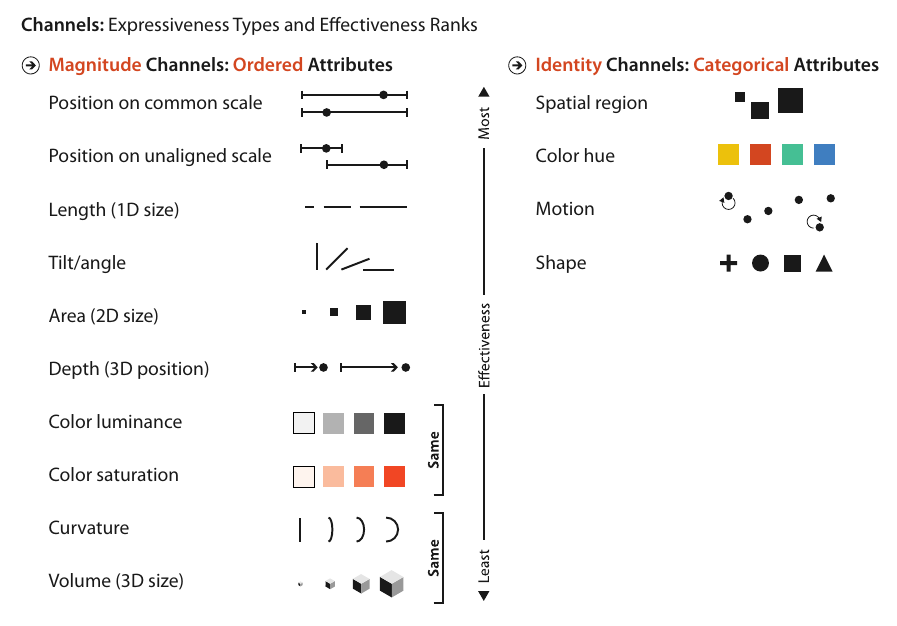
\includegraphics[width=0.5\textwidth]{img/Munzner_Channels.png}
    \caption{The effectiveness of channels that modify the appearance of marks~\cite{munzner_visualization_2014}}
    \label{fig:munzner_channels}
\end{figure}


%------------------------------------
%         End of Content 
%------------------------------------
% insert references
% add the references to the references.bib file
\newpage
\ifeng
 \fancyhead[L]{References}
 \addcontentsline{toc}{section}{References} 
\else
 \fancyhead[L]{Literatur}
 \addcontentsline{toc}{section}{Literatur} 
\fi

\bibliographystyle{plain}
\bibliography{references}


% insert  affidavit / eidesstattliche erklärung
\newpage
\section*{Eidesstattliche Erklärung}
\fancyhead[L]{Eidesstattliche Erklärung}
\addcontentsline{toc}{section}{Eidesstattliche Erklärung} 
Ich erkläre an Eides statt, dass ich die vorliegende {\ifcase\type Dissertation\or Diplomarbeit\or Masterarbeit\or Bachelorarbeit\fi} selbstständig und ohne fremde Hilfe verfasst, andere als die angegebenen Quellen und Hilfsmittel nicht benutzt bzw. die wörtlich oder sinngemäß entnommenen Stellen als solche kenntlich gemacht habe.
Die vorliegende {\ifcase\type Dissertation\or Diplomarbeit\or Masterarbeit\or Bachelorarbeit\fi} ist mit dem elektronisch übermittelten Textdokument identisch.

\vspace{2.5cm}
\parbox{4cm}{\hrule
\strut \footnotesize Ort, Datum} \hfill\parbox{4cm}{\hrule
\strut \footnotesize Unterschrift}

\end{document}
